\documentclass[12pt]{article}

\usepackage{graphicx}
\usepackage{geometry}
\usepackage{setspace}
\usepackage{multirow}
\usepackage[table,xcdraw]{xcolor}
\usepackage{caption}
\usepackage{tocbibind} %Index of table of contents
\usepackage{url} 
\geometry{a4paper, total={170mm, 257mm}, left=20mm, right=20mm, top=25mm, bottom=25mm}
\usepackage[spanish,es-tabla]{babel}

\usepackage{fancyhdr}
\pagestyle{fancy}
\fancyhf{} % Limpia los estilos anteriores de encabezado y pie de página

% Define el contenido del encabezado
\rhead{Tecnológico de Costa Rica}

% Opcional: Puedes personalizar el pie de página si lo necesitas
% \lfoot{Pie de página izquierdo}
\cfoot{\thepage} % Número de página en el centro
% \rfoot{Pie de página derecho}

% Línea horizontal en la parte superior del encabezado
\renewcommand{\headrulewidth}{0.5pt}

\setlength{\parindent}{1em}
\setlength{\parskip}{1em}

\usepackage{makeidx}
\makeindex


%%%%%%%%%%%%%%%%%%%%%%%%%%%%%%%%%%%%%%%%%%%%%%%%%%%%%%%%%%%%%%%%%%%%%%%%%%%%%%%%%%%%%%%%%%%%%%%%%%%%%%%%%%%%%%%%%%%%%% here Begins the document

\begin{document}
\begin{titlepage}

  \centering


  \vspace{10cm}

  \textbf{\LARGE Instituto Tecnológico de Costa Rica}

  \vspace{2cm}

  \textbf{\LARGE Escuela de Ingeniería Electrónica}

  \vspace{2cm}

  
\includegraphics[width=10cm]{logotec/image.png}
  \vspace{2cm}

  \hrule

  \vspace{1cm}

  \textbf{\LARGE Diseño de un sistema para soportar algoritmos de control basados en aprendizaje automático en tiempo real}

  \vspace{1cm}

  \hrule

  \vspace{1cm}

  \textbf{\LARGE SIPLab-TEC}

  \vspace{1cm}

  \textbf{\LARGE David Felipe Duarte Sánchez}

  \vspace{1cm}

  \textbf{\LARGE 2017239606}

  \vspace{1cm}

  \today % Esto agrega la fecha actual

\end{titlepage}
.
\par
\vspace{16cm} % Ajusta la cantidad de espacio vertical según sea necesario

Yo, David Duarte Sánchez portador de la cédula 305070982, declaro que los resultados obtenidos en el presente trabajo de investigación, previo a la obtención del título de Licenciado en Ingeniería en Electrónica, son absolutamente originales, auténticos y personales.

Soy consciente de que el hecho de no respetar los derechos de autor y realizar una mala conducta científica; es decir, fabricación de datos falsos y plagio, conlleva
sanciones universitarias y/o legales.

En tal virtud, declaro que el trabajo de investigación realizado sujeto a evaluación no ha sido presentado anteriormente para obtener algún grado académico o título, ni ha sido publicado en sitio alguno y los efectos legales y académicos que se puedan derivar del trabajo propuesto de investigación son y serán de mí sola y exclusiva responsabilidad legal y académica.

\newpage
%\renewcommand{\contentsname}{Contenidos} commenting due babel integration
\tableofcontents

\newpage

\section{Entorno del proyecto}

El laboratorio de procesamiento de señales e imágenes SIPLab de la Escuela de Electrónica, se enfoca en la solución de problemas de ámbito nacional y regional relacionados con el procesamiento y reconocimiento de información, transportada en señales temporales y espaciales. De momento se trabaja en un proyecto de aplicación del aprendizaje automático en tareas de control automático  \cite{SIPLab} \cite{13_se}.

%La tesis de Jorge Brenes 
Un antecedente a este proyecto, \cite{15_tec} realizó un modelo sustituto neuronal para una planta real y actualmente se está diseñando un modelo de control por inteligencia artificial que debe ejecutarse en tiempo real. Este proyecto pretende proponer el sistema que dé soporte a todo el concepto, de modo que los subsistemas se comuniquen y actúen en tiempo real, bajo consideración de los requisitos que imponga el sistema de control junto a la planta a controlar. 

Los sistemas en tiempo real, son sistemas en los que la respuesta de la aplicación ante estímulos externos debe realizarse dentro de un plazo de tiempo establecido. La predictibilidad del tiempo de respuesta determina si el sistema será capaz de ofrecer una respuesta correcta ante la llegada de un estímulo en un tiempo acotado. Esto permite conocer a priori cuál va a ser el comportamiento del sistema en las peores condiciones y de esta forma realizar un análisis de tiempos de respuesta del sistema \cite{alonso2010panoramica}. En la Figura \ref{fig:diagrama_tiempo_real}, se observa un diagrama descriptivo de la ejecución de una tarea en un sistema de tiempo real, en donde se observan atributos temporales como: activación y plazo de respuesta\cite{de2000introduccion}.

%algunas metricas utilizadas

En el diseño de software del sistema de control, cada uno de los controladores se estructura en una tarea. Hay métodos y herramientas para el diseño, análisis y validación de sistemas de tiempo real caracterizado por el modelo de tareas periódico. Una tarea está caracterizada por parámetros funcionales como \cite{alonso2010panoramica}: 


\textbf{Periodo}: Cada periodo de una tarea es una secuencia de activaciones que se cumplen en un intervalo de tiempo.\\
\textbf{Plazo de entrega}:  Intervalo de tiempo máximo que puede transcurrir desde el instante de activación y la finalización del proceso. Normalmente, es igual al periodo. Cada tarea debe de finalizar la ejecución antes de iniciar el siguiente periodo. \\
\textbf{Desfase inicial}: Desfase entre el inicio de la primera activación respecto al tiempo de inicio.\\
\textbf{Tiempo de procesamiento}: Tiempo necesario para completar la ejecución de cada una de las activaciones. Depende de la complejidad del algoritmo de control y la velocidad del procesador. La ejecución puede variar entre dos límites, mínimo y máximo, el límite máximo es el tiempo de peor caso y será el empleado en el análisis de planificabilidad.\\
\textbf{Retardo de inicio} : Tiempo en el que la actividad comienza a ser ejecutada. Es determinado por el sistema de ejecución y por las decisiones del planificador. \\
\textbf{Tiempo de finalización} : Tiempo que depende del instante de inicio de la ejecución, tiempo de procesamiento y retrasos que sufre al acceder por los datos necesarios y generados por interferencia con otras tareas. \\


\begin{figure}[!ht]
  \centering
  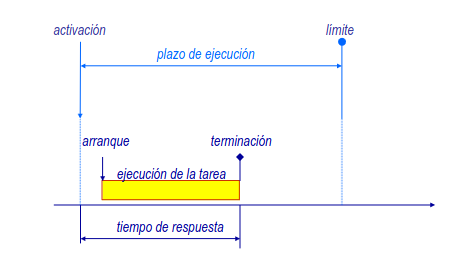
\includegraphics[scale=0.5]{diagramas/tiempo_real.png}
  \caption{Ejecución de una tarea de tiempo real Fuente: \cite{de2000introduccion}}
  \label{fig:diagrama_tiempo_real}
\end{figure}



\newpage

\section{Definición del problema}

\subsection{Generalidades}

Los sistemas en tiempo real son sistemas diseñados para procesar eventos dentro de límites temporales, cumpliendo restricciones definidas. Implican tiempos de respuesta predecibles y deterministas para las tareas del sistema. Emplean algoritmos de planificación de CPU de tiempo real que asignan los recursos de forma óptima. La gestión eficiente de eventos y la sincronización de tareas son aspectos críticos, mientras que la fiabilidad y disponibilidad del sistema se aseguran mediante mecanismos de recuperación de errores y redundancia de hardware y software \cite{de2000introduccion}.

Estos sistemas se dividen en sistemas críticos y acríticos. Los sistemas críticos son aquellos en los que las acciones del sistema se deben de producir dentro del plazo de ejecución de la tarea. De no cumplir la tarea en el plazo establecido, ocurren fallos en la operación del sistema y perdida de datos. Se pueden encontrar en sistemas aeronáuticos, control de satélites y procesos industriales. Por otro lado, en los sistemas acríticos la perdida o retraso en alguno de los plazos ocasiona que el sistema tenga una degradación durante algunos ciclos de operación, para luego recuperarse y continuar operando de forma normal \cite{de2000introduccion} \cite{alonso2010panoramica}.

Por otro lado, los sistemas en tiempo real son aplicados en el control automático por la capacidad de procesar información y responder en un instante definido ante cambios en el entorno o condiciones del sistema. En aplicaciones donde la rapidez y precisión son esenciales, estos sistemas garantizan  una supervisión y regulación continua y efectiva. Su capacidad en la toma de decisiones en tiempo real no solo mejora la eficiencia operativa, si no, también disminuye el riesgo de fallos y errores contribuyendo a la seguridad del sistema \cite{munoz1994extensiones}. 

Las plataformas en tiempo real para aplicaciones en control automático, se implementan en SoC de alto rendimiento tomando en cuenta que un manejo eficiente del entorno en tiempo real tiene la capacidad de acelerar las diversas tareas de control. También se deben garantizar las restricciones temporales para ejecutar las actividades en tiempo real y asegurar que el sistema operativo tenga un comportamiento predecible. Para garantizar el cumplimiento de las restricciones es necesario realizar un análisis que permita conocer si las restricciones impuestas se van a cumplir en cualquier situación. Esto se realiza en función de cómo y cuándo se toman las decisiones de planificación. Se dividen en dos grupos, Off-Line, lo que indica que las decisiones se tomaron en la etapa de diseño y On Line cuando las decisiones se toman durante la ejecución \cite{munoz1994extensiones} \cite{alonso2010panoramica}.


\subsection{Síntesis del problema}

El SIPLab no cuenta con un marco de trabajo que permita ejecutar controladores neuronales en tiempo real sobre sistemas embebidos heterogéneos, que sea configurable y que cuente con mecanismos de medición de su desempeño.


\section{Enfoque de la solución}

Se debe de proponer como solución una plataforma de trabajo para un sistema embebido que logre ejecutar en tiempo real un sistema de control automático neuronal.


Con una matriz de Pugh se analizan caminos de solución, con el objetivo de seleccionar aquella más adecuada, en donde un cero indica que una alternativa es similar, un +1 que la alternativa es mejor o un -1 que la alternativa es peor, comparada a la referencia.

\subsection{Alternativa 1}

%Diseñar una plataforma de trabajo para un sistema embebido que logre ejecutar en tiempo real un sistema de control automático neuronal.

Se plantea el diseño de una plataforma de trabajo para un sistema embebido, que logre ejecutar en tiempo real, un sistema de control automático neuronal mediante un acelerador de hardware. Para esta alternativa se propone el uso de un sistema propietario, un hardware dedicado que funciona con un software propietario para mejorar el rendimiento de tareas\cite{zhao2017hardware} \cite{shi2011vcuda}, Mediante el uso de unidades de procesamiento tensorial con el fin de acelerar operaciones de aprendizaje automático. Utilizando estos sistemas se obtiene un rendimiento optimizado, ya que trabajan de forma eficiente y optimizada con el hardware específico, también una integración profunda lo cual facilita el desarrollo, por tanto, tienden a ser sistemas más rápidos, finalmente, los sistemas propietarios en algunos casos proveen soporte del fabricante. Por otro lado, experimentan bloqueos de proveedor, lo que limita la flexibilidad e interoperabilidad de interactuar con otros sistemas \cite{deng2020model} \cite{duato2011enabling}.

\subsection{Alternativa 2}

Se plantea el diseño de una plataforma de trabajo para un sistema embebido, que logre ejecutar en tiempo real, un sistema de control automático neuronal mediante un acelerador de hardware. En este caso se propone el uso de un sistema abierto, buscando mejorar el rendimiento y la eficiencia de los sistemas mediante la utilización de hardware especializado, pero garantizando que el desarrollo y diseño sea abierto \cite{scarpino2011opencl} \cite{owaida2011massively}. El uso de las unidades de procesamiento tensorial permite acelerar las operaciones de aprendizaje automático, el controlador neuronal y mejorar los parámetros de tasa de muestreo, jitter de entrada y jitter de salida. Además, permite tener más transparencia al operar con el sistema, tomando en cuenta la flexibilidad del sistema y personalización permitiendo la adaptación del hardware a necesidades específicas y el costo reducido al implementar esta alternativa. Por otro lado, los sistemas abiertos no presentan soporte por parte del fabricante, también no siempre van a proporcionar el mismo nivel de rendimiento que las soluciones propietarias \cite{meyer2020evaluating} \cite{verma2016accelerating}.

\subsection{Alternativa 3}
Se plantea el diseño de una plataforma de trabajo para un sistema embebido, que logre ejecutar en tiempo real, un sistema de control automático neuronal mediante aceleración de software, mejorando de esta forma la eficiencia y velocidad de ejecución \cite{galan2000control}. Mediante variables como la optimización de código, paralelización de tareas e implementando técnicas de caché y preprocesamiento. Se podrá tener una respuesta rápida y optimización de recursos. Por otro lado, aspectos como fallos críticos y limitantes a nivel de hardware son algunas de las desventajas de esta implementación \cite{kim1994software} \cite{razdan1994prisc}.


\subsection{Selección de la solución}

Matriz de pugh que compara las 3 alternativas Cuadro \ref{tab:pugh}.

% Please add the following required packages to your document preamble:
% \usepackage[table,xcdraw]{xcolor}
% Beamer presentation requires \usepackage{colortbl} instead of \usepackage[table,xcdraw]{xcolor}
\begin{table}[!h]
% Please add the following required packages to your document preamble:

  \centering
  \caption{Matriz de Pugh para la selección de la solución}
  \label{tab:pugh}
  \begin{tabular}{ccccc}
  \cline{2-5}
  \multicolumn{1}{l|}{} & \multicolumn{1}{c|}{\cellcolor[HTML]{DAE8FC}} & \multicolumn{1}{c|}{\cellcolor[HTML]{DAE8FC}} & \multicolumn{1}{c|}{\cellcolor[HTML]{DAE8FC}} & \multicolumn{1}{c|}{\cellcolor[HTML]{DAE8FC}} \\ \cline{1-1}
  \rowcolor[HTML]{DAE8FC} 
  \multicolumn{1}{|c|}{\cellcolor[HTML]{DAE8FC}Criterios} & \multicolumn{1}{c|}{\multirow{-2}{*}{\cellcolor[HTML]{DAE8FC}Peso}} & \multicolumn{1}{c|}{\multirow{-2}{*}{\cellcolor[HTML]{DAE8FC}Alternativa 1}} & \multicolumn{1}{c|}{\multirow{-2}{*}{\cellcolor[HTML]{DAE8FC}Alternativa 2}} & \multicolumn{1}{c|}{\multirow{-2}{*}{\cellcolor[HTML]{DAE8FC}Alternativa 3}} \\ \hline
  \multicolumn{1}{|c|}{\cellcolor[HTML]{DAE8FC}\begin{tabular}[c]{@{}c@{}}Transparencia de \\ operación\end{tabular}} & \multicolumn{1}{c|}{\cellcolor[HTML]{CBCEFB}3} & \multicolumn{1}{c|}{-1} & \multicolumn{1}{c|}{+1} & \multicolumn{1}{c|}{=} \\ \hline
  \multicolumn{1}{|c|}{\cellcolor[HTML]{DAE8FC}\begin{tabular}[c]{@{}c@{}}Flexibilidad y\\ Personalización\end{tabular}} & \multicolumn{1}{c|}{\cellcolor[HTML]{CBCEFB}5} & \multicolumn{1}{c|}{-1} & \multicolumn{1}{c|}{+1} & \multicolumn{1}{c|}{=} \\ \hline
  \multicolumn{1}{|c|}{\cellcolor[HTML]{DAE8FC}\begin{tabular}[c]{@{}c@{}}Costo de \\ implementación\end{tabular}} & \multicolumn{1}{c|}{\cellcolor[HTML]{CBCEFB}5} & \multicolumn{1}{c|}{-1} & \multicolumn{1}{c|}{+1} & \multicolumn{1}{c|}{=} \\ \hline
  \multicolumn{1}{|c|}{\cellcolor[HTML]{DAE8FC}Rendimiento} & \multicolumn{1}{c|}{\cellcolor[HTML]{CBCEFB}5} & \multicolumn{1}{c|}{+1} & \multicolumn{1}{c|}{+1} & \multicolumn{1}{c|}{-1} \\ \hline
  \multicolumn{1}{|c|}{\cellcolor[HTML]{DAE8FC}Mantenibilidad} & \multicolumn{1}{c|}{\cellcolor[HTML]{CBCEFB}4} & \multicolumn{1}{c|}{+1} & \multicolumn{1}{c|}{-1} & \multicolumn{1}{c|}{-1} \\ \hline
  \multicolumn{1}{|c|}{\cellcolor[HTML]{DAE8FC}Innovación} & \multicolumn{1}{c|}{\cellcolor[HTML]{CBCEFB}5} & \multicolumn{1}{c|}{+1} & \multicolumn{1}{c|}{+1} & \multicolumn{1}{c|}{-1} \\ \hline
  \multicolumn{1}{|c|}{\cellcolor[HTML]{DAE8FC}\begin{tabular}[c]{@{}c@{}}Porteabilidad de \\ la solución\end{tabular}} & \multicolumn{1}{c|}{\cellcolor[HTML]{CBCEFB}4} & \multicolumn{1}{c|}{-1} & \multicolumn{1}{c|}{+1} & \multicolumn{1}{c|}{-1} \\ \hline
  \multicolumn{1}{|c|}{\cellcolor[HTML]{DAE8FC}\begin{tabular}[c]{@{}c@{}}Ajuste de \\ parámetros\end{tabular}} & \multicolumn{1}{c|}{\cellcolor[HTML]{CBCEFB}5} & \multicolumn{1}{c|}{+1} & \multicolumn{1}{c|}{+1} & \multicolumn{1}{c|}{+1} \\ \hline
  \multicolumn{1}{|c|}{\cellcolor[HTML]{DAE8FC}\begin{tabular}[c]{@{}c@{}}Ejecución en \\ tiempo real\end{tabular}} & \multicolumn{1}{c|}{\cellcolor[HTML]{CBCEFB}5} & \multicolumn{1}{c|}{+1} & \multicolumn{1}{c|}{+1} & \multicolumn{1}{c|}{-1} \\ \hline
  \multicolumn{1}{l}{} & \multicolumn{1}{l}{} & \multicolumn{1}{l}{} & \multicolumn{1}{l}{} & \multicolumn{1}{l}{} \\ \cline{1-1} \cline{3-5} 
  \multicolumn{1}{|c|}{\cellcolor[HTML]{DAE8FC}Suma General} & \multicolumn{1}{c|}{} & \multicolumn{1}{c|}{4} & \multicolumn{1}{c|}{36} & \multicolumn{1}{c|}{-13} \\ \cline{1-1} \cline{3-5} 
  \multicolumn{1}{|c|}{\cellcolor[HTML]{DAE8FC}Posición} & \multicolumn{1}{c|}{} & \multicolumn{1}{c|}{2} & \multicolumn{1}{c|}{1} & \multicolumn{1}{c|}{3} \\ \cline{1-1} \cline{3-5} 
  \end{tabular}
  \end{table}


Cuando se realiza el análisis de la Matriz de Pugh se puede determinar que en aspectos como lo son ajustes de parámetros o innovación la alternativa 2 y 3 se encuentran empatadas, ya que hay que recordar que lo que difiere entre estas dos opciones es el método de implementación, por un lado, en la alternativa 2 se propone el uso de un software agnóstico de hardware como base del diseño mientras que en la alternativa 3 se plantea el uso de un método en software, eliminando virtudes de la alternativa 2 y 1 como lo era la velocidad de procesamiento de datos. Es por esto que criterios como lo fueron la ejecucion en tiempo real, rendimiento e innovación terminaron de inclinar la balanza por el uso de la alternativa 2.

\section{Objetivo General}

Diseñar una plataforma de trabajo para un sistema embebido que logre ejecutar en tiempo real un sistema de control automático neuronal el cual cumpla con las métricas especificadas en la tabla \ref{tab:obj_1}.

\textbf{Indicador:} Cumplir al menos un 90 \% de las métricas especificadas en la tabla \ref{tab:obj_1}.\newline
\textbf{Entregable:} Resumen de los resultadosd e todo el proceso de desarrollo e implementacion de una plataforma de trabajo para un sistema embebido que logre ejecutar en tiempo real un sistema de control automático en tiempo real.


\begin{table}[!h]
  \centering
  \caption{Requisitos para satisfacer el indicador del objetivo general}
  \label{tab:obj_1}
  \begin{tabular}{|l|}
    \hline
    \rowcolor[HTML]{DAE8FC} 
    Requisitos \\ \hline
    Latencia menor a 50 ms\\ \hline
    Tasa de éxito de transmisión de al menos un 90\%\\ \hline
    Precisión de los datos (Error absoluto medio MAE del 5\%)\\ \hline
    Saturacion del sistema no mayor al 90\% \\ \hline
    Tiempo de procesamiento menor o igual a \\ 20ms por muestra recibida\\ \hline
    \end{tabular}
\end{table}

\section{Objetivos Específicos}

\begin{enumerate}
  \item Investigar acerca de plataformas que garantizen que el análisis de los datos se de en tiempo real. \newline
        \textbf{Indicador:} Se genera una matriz de Pugh con al menos 6 criterios.\newline
        \textbf{Entregable:} Matriz de Pugh con al menos 6 criterios a evaluar y la plataforma seleccionada.
  \item Implementar la plataforma seleccionada \newline
        \textbf{Indicador:} Plataforma cumple con los requisitos del Cuadro \ref{tab:obj_1}.\newline
        \textbf{Entregable:} El sistema implementado.
  \item Evaluar la plataforma seleccionada \newline
        \textbf{Indicador:} Se evaluan al menos 3 configuraciones del sistema y se utilizan al menos 3 métricas para la evaluación del desempeño de las mismas.\newline
        \textbf{Entregable:} Documentación de la evaluación cuantitativa del sistema en el documento de tesis.
\end{enumerate}

\section{Procedimiento para la ejecución del proyecto}

Sobre la ejecución del proyecto se planifican las actividades de forma jerárquica, en donde se establecen actividades según los objetivos planteados, los requisitos de las actividades y la dependencia que tenga este mismo con alguna actividad previa. Además de esto se definen los tiempos de duración de las actividades las cuales se resumen en el Cuadro \ref{tab:actividades}.

% Please add the following required packages to your document preamble:
% \usepackage{multirow}
\begin{table}[ht]
  \centering
  \caption{Procedimiento para la ejecución del proyecto}
  \label{tab:actividades}
  \begin{tabular}{|c|c|c|c|}
    \hline
    Objetivo                                                                                                                                                                  & Actividad                                                                                                                      & Tiempo en días & Dependencias \\ \hline
    \multirow{4}{*}{\begin{tabular}[c]{@{}l@{}} 1.Investigar acerca de \\ plataformas que \\ garantizen que el análisis \\ de los datos \\ se dé en tiempo real.\end{tabular}} & \begin{tabular}[c]{@{}l@{}}1.1 Investigar sobre \\ sistemas en tiempo \\ real.\end{tabular}                                    & 5            &              \\ \cline{2-4}
                                                                                                                                                                              & \begin{tabular}[c]{@{}l@{}}1.2 Investigar sobre \\ análisis de datos en \\ tiempo real.\end{tabular}                           & 5             & 1.1          \\ \cline{2-4}
                                                                                                                                                                              & \begin{tabular}[c]{@{}l@{}}1.3 Definir los criterios \\ del sistema de tiempo \\ real.\end{tabular}                            & 5              & 1.2          \\ \cline{2-4}
                                                                                                                                                                              & \begin{tabular}[c]{@{}l@{}}1.4 Elección del\\ sistema.\\ del sistema de tiempo \\ real.\end{tabular}                            & 8              & 1.2          \\ \cline{2-4}
                                                                                                                                                                              & \begin{tabular}[c]{@{}l@{}}1.5 Documentación de los datos \end{tabular}                                                         & 8              & 1.4          \\ \hline
    \multicolumn{1}{|l|}{\multirow{2}{*}{\begin{tabular}[c]{@{}l@{}}2. Implementar la plataforma \\ seleccionada.\end{tabular}}}                                              & \begin{tabular}[c]{@{}l@{}}2.1 Implementación del \\ sistema seleccionado.\end{tabular}                                        & 15             & 1.4          \\ \cline{2-4}
    \multicolumn{1}{|l|}{}                                                                                                                                                    & \begin{tabular}[c]{@{}l@{}}2.2 Evaluación de los \\ parámetros seleccionados\\  en el sistema.\end{tabular}                    & 8             & 2.1          \\ \cline{2-4}
    \multicolumn{1}{|l|}{}                                                                                                                                                    & \begin{tabular}[c]{@{}l@{}}2.3 Documentación de los datos.\end{tabular}                    & 8             & 2.2          \\ \hline
    \multicolumn{1}{|l|}{\multirow{2}{*}{\begin{tabular}[c]{@{}l@{}}3. Evaluar la plataforma \\ seleccionada\end{tabular}}}                                                   & \begin{tabular}[c]{@{}l@{}}3.1 Evaluación de las \\ configuraciones del \\ sistema.\end{tabular}                               & 10            & 2.2          \\ \cline{2-4}
    \multicolumn{1}{|l|}{}                                                                                                                                                    & \begin{tabular}[c]{@{}l@{}}3.2 Selección de \\ las métricas \\ para evaluar el \\ rendimiento del \\ sistema.\end{tabular} & 2            & 3.1          \\ \cline{2-4}
    \multicolumn{1}{|l|}{}                                                                                                                                                    & \begin{tabular}[c]{@{}l@{}}3.3 Evaluación del \\ desempeño del sistema \\ mediante las métricas \\ seleccionadas.\end{tabular} & 3            & 3.2          \\ \cline{2-4}
    \multicolumn{1}{|l|}{}                                                                                                                                                    & \begin{tabular}[c]{@{}l@{}}3.4 Documentación de los datos. \end{tabular} & 5            & 3.3          \\ \hline    
  \end{tabular}
\end{table}


\section{Cronograma de actividades}

La agenda de actividades según el tiempo asignado comprende desde el  5 de febrero del 2024 hasta el 25 de mayo del 2024, tiempo el cual abarca 16 semanas lectivas en las cuales se llevara a cabo el desarrollo del proyecto. Por un lado, el cronograma se presenta como un diagrama de Gantt. El mismo ilustra en la Figura \ref{fig:gantt}. Por otro lado, en la Figura \ref{fig:pert} se muestra el diagrama de PERT con las dependencias entre actividades.

\newpage

\begin{figure}
  \centering
  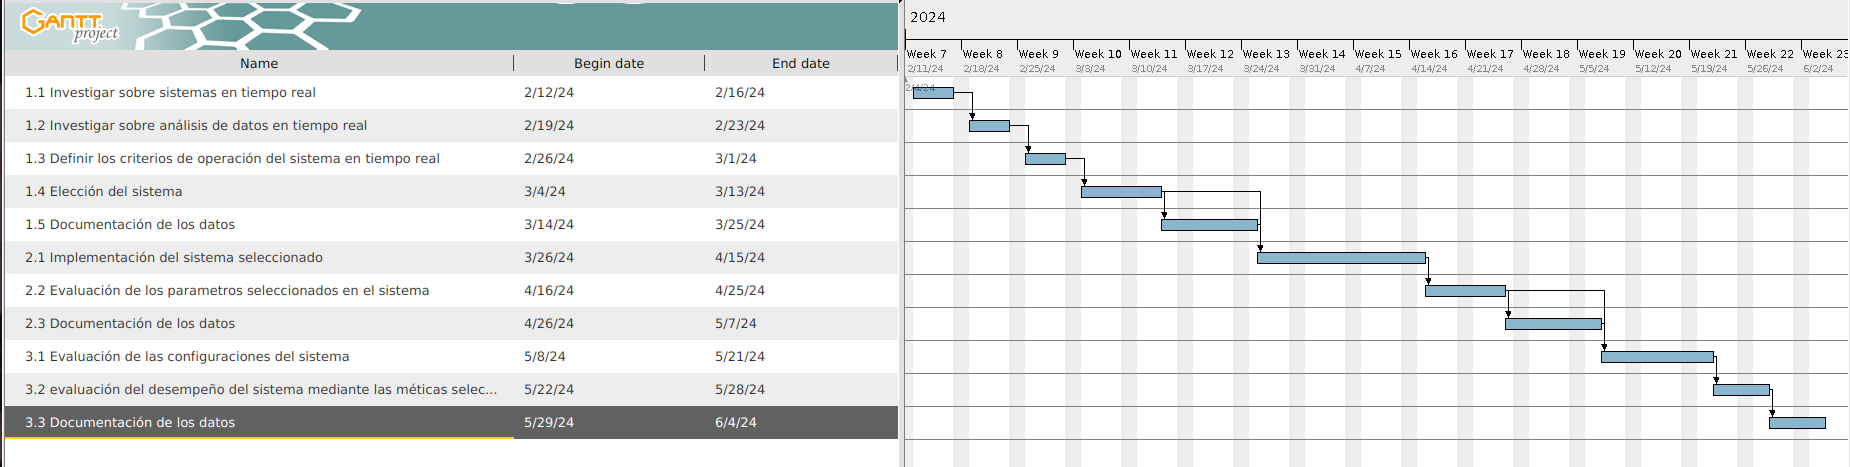
\includegraphics[scale=0.3, angle=90]{diagramas/gantt.png}
  \caption{Ruta critica del cronograma de actividades}
  \label{fig:gantt}
\end{figure}

\begin{figure}
  \centering
  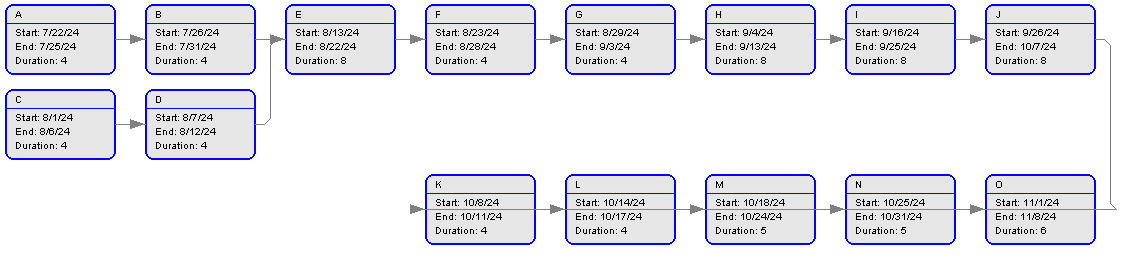
\includegraphics[scale=0.3, angle=90]{diagramas/pert.png}
  \caption{Diagrama PERT de las actividades}
  \label{fig:pert}
\end{figure}


\subsection{Entregables}

Como se puede observar en el Cuadro \ref{tab:entregables} se encuentra una lista de los entregables con sus objetivos y fechas de entrega establecidas en el periodo donde se llevara a cabo el trabajo final de graduación.

\begin{table}[ht]
  \centering
  \caption{Lista de entregables}
  \label{tab:entregables}
  \begin{tabular}{|l|l|l|}
    \hline
    Objetivo         & Entregable                                                                                                                                                                & Fecha de entrega \\ \hline
    Específico 1     & \begin{tabular}[c]{@{}l@{}}Matriz de Pugh con al menos \\ 6 criterios a evaluar del sistema \\ en tiempo real y el sistema \\ seleccionado.\end{tabular}                  &   25/3/2024       \\ \hline
    Específico 2     & El sistema implementado                                                                                                                                                   &   7/5/2024      \\ \hline
    Específico 3     & \begin{tabular}[c]{@{}l@{}}Métricas de calidad en donde \\ se define cuál confuiguración \\ es mejor según la métrica \\ seleccionada.\end{tabular}                       &   21/5/2024      \\ \hline
    Objetivo general & \begin{tabular}[c]{@{}l@{}}Plataforma de trabajo en tiempo\\ real para un sistema embebido\\ que logre ejecutar un sistema de \\ control automático neuronal\end{tabular} &   4/6/2024      \\ \hline
  \end{tabular}
\end{table}


\section{Uso de recursos}

Para ejecutar el software encargado de controlar la planta prototipo por medio de aprendizaje reforzado se hace uso de la siguiente lista de materiales.

\begin{itemize}
  \item Una planta prototipo de control automático donde se implemente el controlador.
  \item Computadora donde desarrollar el controlador. En caso de ser portátil, se requiere accesorios como el cargador.
  \item Tarjeta de desarrollo NVIDIA Jetson TX2.
  \item Acceso a internet para llevar a cabo la revisión bibliográfica.
\end{itemize}

\newpage

\section{Presupuesto}

Se realiza la estimación del presupuesto. 

\begin{figure}[ht]
  \centering
  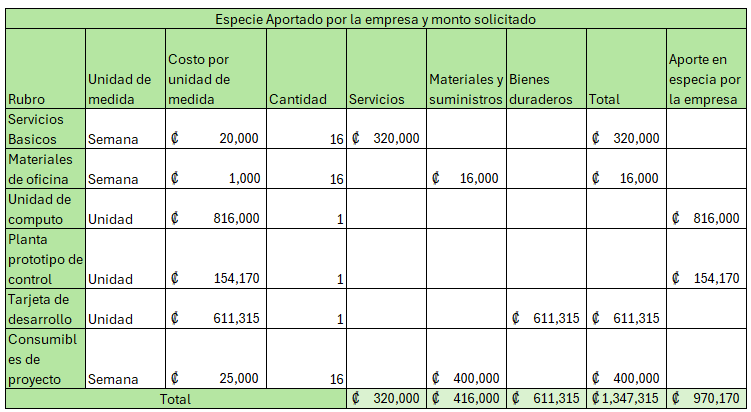
\includegraphics[scale=0.8]{tablas/ptot.png}
  \captionsetup{labelformat=empty}  % Eliminar la etiqueta predeterminada ("Figura")
  \caption{Tabla 4: Presupuesto para realizar el proyecto}
\end{figure}

\begin{figure}[ht]
  \centering
  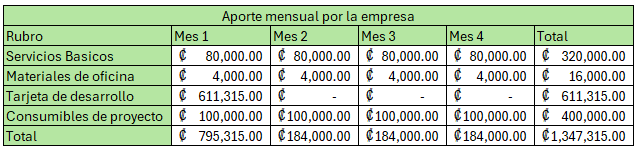
\includegraphics[scale=0.8]{tablas/pmensual.png}
  \captionsetup{labelformat=empty}  % Eliminar la etiqueta predeterminada ("Figura")
  \caption{Tabla 5: Presupuesto Mensual para realizar el proyecto}
\end{figure}


\newpage

\bibliography{biblio.bib}
\bibliographystyle{plain}

\end{document}